\chapter{Introduction}
\section{The concept of attack}

To effectively understand attacks on the different services, we should look at
how these services can be attacked. A concept is an outlined plan that is
applied to future projects. 

we can try to group the services SSH, FTP, SMB, and HTTP ourselves and figure
out what these services have in common. Then we need to create a structure that
will allow us to identify the attack points of these different services using a
single pattern.

Analyzing commonalities and creating pattern templates that fit all conceivable
cases is not a finished product but rather a process that makes these pattern
templates grow larger and larger. Therefore, we have created a pattern template
for this topic for you to better and more efficiently teach and explain the
concept behind the attacks.

\begin{figure}
  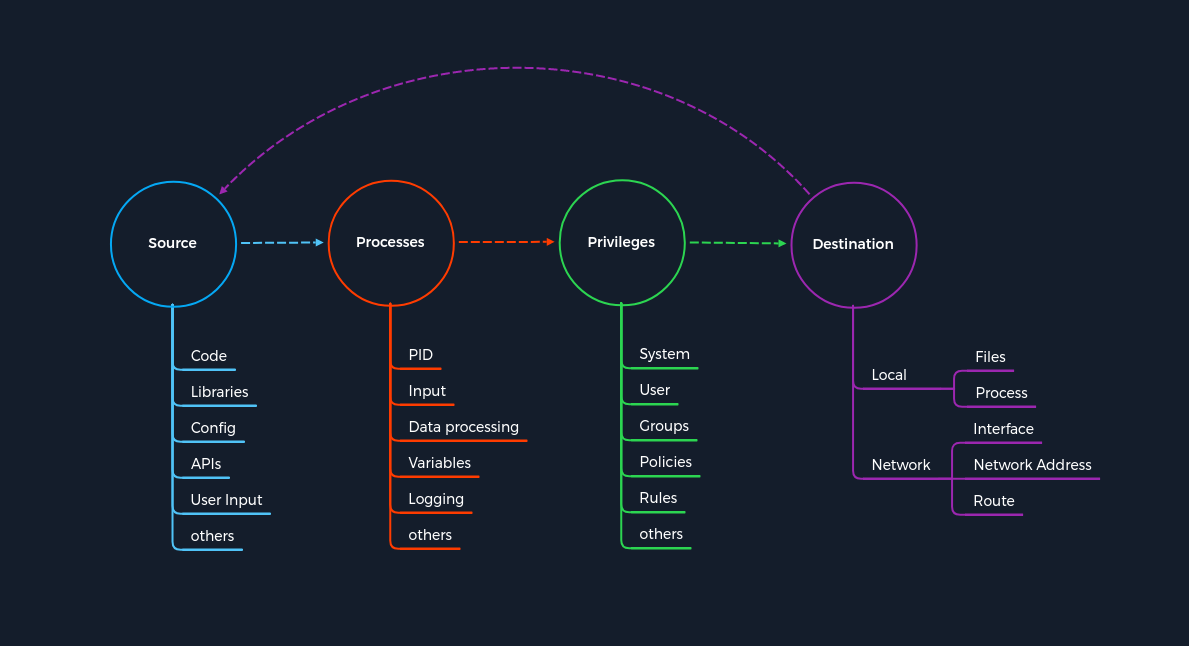
\includegraphics[width=\linewidth]{network/intro/images/attack_concept.png}
  \caption{Attack concept}
  \label{fig:attack_concept}
\end{figure}
The concept is based on four categories that occur for each vulnerability.
First, the {\bf Source} that performs the specific request to a {\bf Process}
where the vulnerability gets triggered. Each process has a specific set of {\bf
Privileges} with which it is executed. Each process has a task with a specific
goal or {\bf Destination} to either compute new data or forward it. However,
the individual and unique specifications under these categories may differ from
service to service.

Every task and piece of information follows a specific pattern, a cycle, which
we have deliberately made linear. This is because the {\bf Destination} does
not always serve as a {\bf Source} and is therefore not treated as a source of
a new task.

For any task to come into existence at all, it needs an idea, information
(Source), a planned process for it (Processes), and a specific goal
(Destination) to be achieved. Therefore, the category of Privileges is
necessary to control information processing appropriately.

\subsection{Source}
Source can be generalized  as a source of information used for the specific
task of a process. There are many different ways to pass information to a
process. The graphic shows some of the most common examples of how information
is passed to the processes.

The source is, therefore, the source that is exploited for vulnerabilities. It
does not matter which protocol is used because HTTP header injections can be
manipulated manually, as can buffer overflows. The source for this can
therefore be categorized as Code. So let us take a closer look at the pattern
template based on
\href{https://cve.mitre.org/cgi-bin/cvename.cgi?name=cve-2021-44228}{Log4j}.



Log4j is a framework or Library used to log application messages in Java and
other programming languages. This library contains classes and functions that
other programming languages can integrate. For this purpose, information is
documented, similar to a logbook. Furthermore, the scope of the documentation
can be configured extensively. As a result, it has become a standard within
many open source and commercial software products. In this example, an attacker
can manipulate the HTTP User-Agent header and insert a JNDI lookup as a command
intended for the Log4j library. Accordingly, not the actual User-Agent header,
such as Mozilla 5.0, is processed, but the JNDI lookup.


\subsection{Process}
The Process is about processing the information forwarded from the source.
These are processed according to the intended task determined by the program
code. For each task, the developer specifies how the information is processed.
This can occur using classes with different functions, calculations, and loops.
The variety of possibilities for this is as diverse as the number of developers
in the world. Accordingly, most of the vulnerabilities lie in the program code
executed by the process.

The process of Log4j is to log the User-Agent as a string using a function and
store it in the designated location. The vulnerability in this process is the
misinterpretation of the string, which leads to the execution of a request
instead of logging the events. However, before we go further into this
function, we need to talk about privileges.

\subsection{Privileges}
Privileges are present in any system that controls processes. These serve as a
type of permission that determines what tasks and actions can be performed on
the system. These privileges can also be used for different means. In computer
systems, these privileges serve as control and segmentation of actions for
which different permissions, controlled by the system, are needed. Therefore,
the rights are checked based on this categorization when a process needs to
fulfill its task. If the process satisfies these privileges and conditions, the
system approves the action requested.

What made the Log4j vulnerability so dangerous was the Privileges that the
implementation brought. Logs are often considered sensitive because they can
contain data about the service, the system itself, or even customers.
Therefore, logs are usually stored in locations that no regular user should be
able to access. Accordingly, most applications with the Log4j implementation
were run with the privileges of an administrator. The process itself exploited
the library by manipulating the User-Agent so that the process misinterpreted
the source and led to the execution of user-supplied code.

\subsection{Destination}

Every task has at least one purpose and goal that must be fulfilled. Logically,
if any data set changes were missing or not stored or forwarded anywhere, the
task would be generally unnecessary. The result of such a task is either stored
somewhere or forwarded to another processing point. Therefore we speak here of
the Destination where the changes will be made. Such processing points can
point either to a local or remote process. Therefore, at the local level, local
files or records may be modified by the process or be forwarded to other local
services for further use. However, this does not exclude the possibility that
the same process could reuse the resulting data too. If the process is
completed with the data storage or its forwarding, the cycle leading to the
task's completion is closed.

The misinterpretation of the User-Agent leads to a JNDI lookup which is
executed as a command from the system with administrator privileges and queries
a remote server controlled by the attacker, which in our case is the
Destination in our concept of attacks. This query requests a Java class created
by the attacker and is manipulated for its own purposes. The queried Java code
inside the manipulated Java class gets executed in the same process, leading to
a remote code execution (RCE) vulnerability.


\section{Misconfiguration}
Some of the most typical misconfigurations of common services
\subsection{Authentication: default / weak}
In previous years (though we still see this sometimes during assessments), it
was widespread for services to include default credentials (username and
password). Nowadays, most software asks users to set up credentials upon
installation, which is better than default credentials. However, keep in mind
that we will still find vendors using default credentials, especially on older
applications.

Even when the service does not have a set of default credentials, an
administrator may use weak passwords or no passwords when setting up services
with the idea that they will change the password once the service is set up and
running.

As administrators, we need to define password policies that apply to software
tested or installed in our environment. Administrators should be required to
comply with a minimum password complexity to avoid weak user and passwords
combinations.

Once the service banner is grabed, the next step should be to identify possible
default credentials. If there are no default credentials, weak username and
password combinations could be tryed.

\subsection{Authentication: anonymous}
Another misconfiguration that can exist in common services is anonymous
authentication. The service can be configured to allow anonymous
authentication, allowing anyone with network connectivity to the service
without being prompted for authentication.

\subsection{Misconfigured Access Rights}

Misconfigured access rights are when user accounts have incorrect permissions.
The bigger problem could be giving people lower down the chain of command
access to private information that only managers or administrators should
have.

Administrators need to plan their access rights strategy, and there are some
alternatives such as
\href{https://en.wikipedia.org/wiki/Role-based_access_control}{Role-based
access control (RBAC)},
\href{https://en.wikipedia.org/wiki/Access-control_list}{Access control lists
(ACL)}. Read
\href{https://authress.io/knowledge-base/role-based-access-control-rbac}{Choosing
the best access control strategy} for pros and cons of each method.
\subsection{Unnecessary Defaults}
The initial configuration of devices and software may include but is not
limited to settings, features, files, and credentials. Those default values are
usually aimed at usability rather than security. Leaving it default is not a
good security practice for a production environment. Unnecessary defaults are
those settings we need to change to secure a system by reducing its attack
surface.

We might as well deliver up our company's personal information on a silver
platter if we take the easy road and accept the default settings while setting
up software or a device for the first time. In reality, attackers may obtain
access credentials for specific equipment or abuse a weak setting by conducting
a short internet search.

Security Misconfiguration are part of the OWASP Top 10 list. Let's take a look
at those related to default values:
\begin{itemize}
    \item  Unnecessary features are enabled or installed (e.g., unnecessary ports, services, pages, accounts, or privileges).
    \item  Default accounts and their passwords are still enabled and unchanged.
    \item  Error handling reveals stack traces or other overly informative error messages to users.
    \item  For upgraded systems, the latest security features are disabled or not configured securely.
\end{itemize}

\section{Sensitive information}

When attacking a service, we usually play a detective role, and we need to
collect as much information as possible and carefully observe the details.
Therefore, every single piece of information is essential.

Let us imagine we are in an engagement with a client, we are targeting email,
FTP, databases, and storage, and our goal is to obtain Remote Code Execution
(RCE) on any of these services. We started the enumeration and tried anonymous
access to all services, and only FTP has anonymous access. We found an empty
file within the FTP service, but with the name johnsmith, we tried johnsmith as
the FTP user and password, but it did not work. We try the same against the
email service, and we successfully login. With email access, we start searching
emails containing the word password, we find many, but one of them contains
John's credentials for the MSSQL database. We access the database and use the
built-in functionality to execute commands and successfully get RCE on the
database server. We successfully met our goal.

A misconfigured service let us access a piece of information that initially may
look insignificant, johnsmith, but that information opened the doors for us to
discover more information and finally get remote code execution on the database
server. This is the importance of paying attention to every piece of
information, every detail, as we enumerate and attack common services.a

Sensitive information may include, but is not limited to:
\begin{itemize}
    \item  Usernames.
    \item  Email Addresses.
    \item  Passwords.
    \item  DNS records.
    \item  IP Addresses.
    \item  Source code.
    \item  Configuration files.
    \item  PII (Personal Identifiable Information).
\end{itemize}


Every target is unique, and we need to familiarize ourselves with our target,
its processes, procedures, business model, and purpose. Once we understand our
target, we can think about what information is essential for them and what kind
of information is helpful for our attack.

There are two key elements to finding sensitive information:
\begin{itemize}
        \item understand the service and how it works.
        \item know what to look for.
\end{itemize}

